% vim: set tw=78 sts=2 sw=2 ts=8 aw et ai:

\subsection{SNM Message Header}
\label{sub-sec:snm-header}
\labelindexref{Fig.}{img:snm-hdr} shows the header used in all SNM messages. \emph{Type} field holds an 1-byte value representing the message type. Current message types values are:
\begin{itemize}
\item \emph{0x01} – for SNM requests
\item \emph{0x02} – for SNM responses
\item \emph{0x03} – for SNM advertise messages
\end{itemize}
A message holding any other message type will be ignored. \emph{Flags} is a 1-byte value representing the flags associated with each message type. On every request, a 2-bytes \emph{Sequence Number} is generated by the issuer for keeping track of all sent messages.

\begin{figure}[hbtp]
\begin{center}
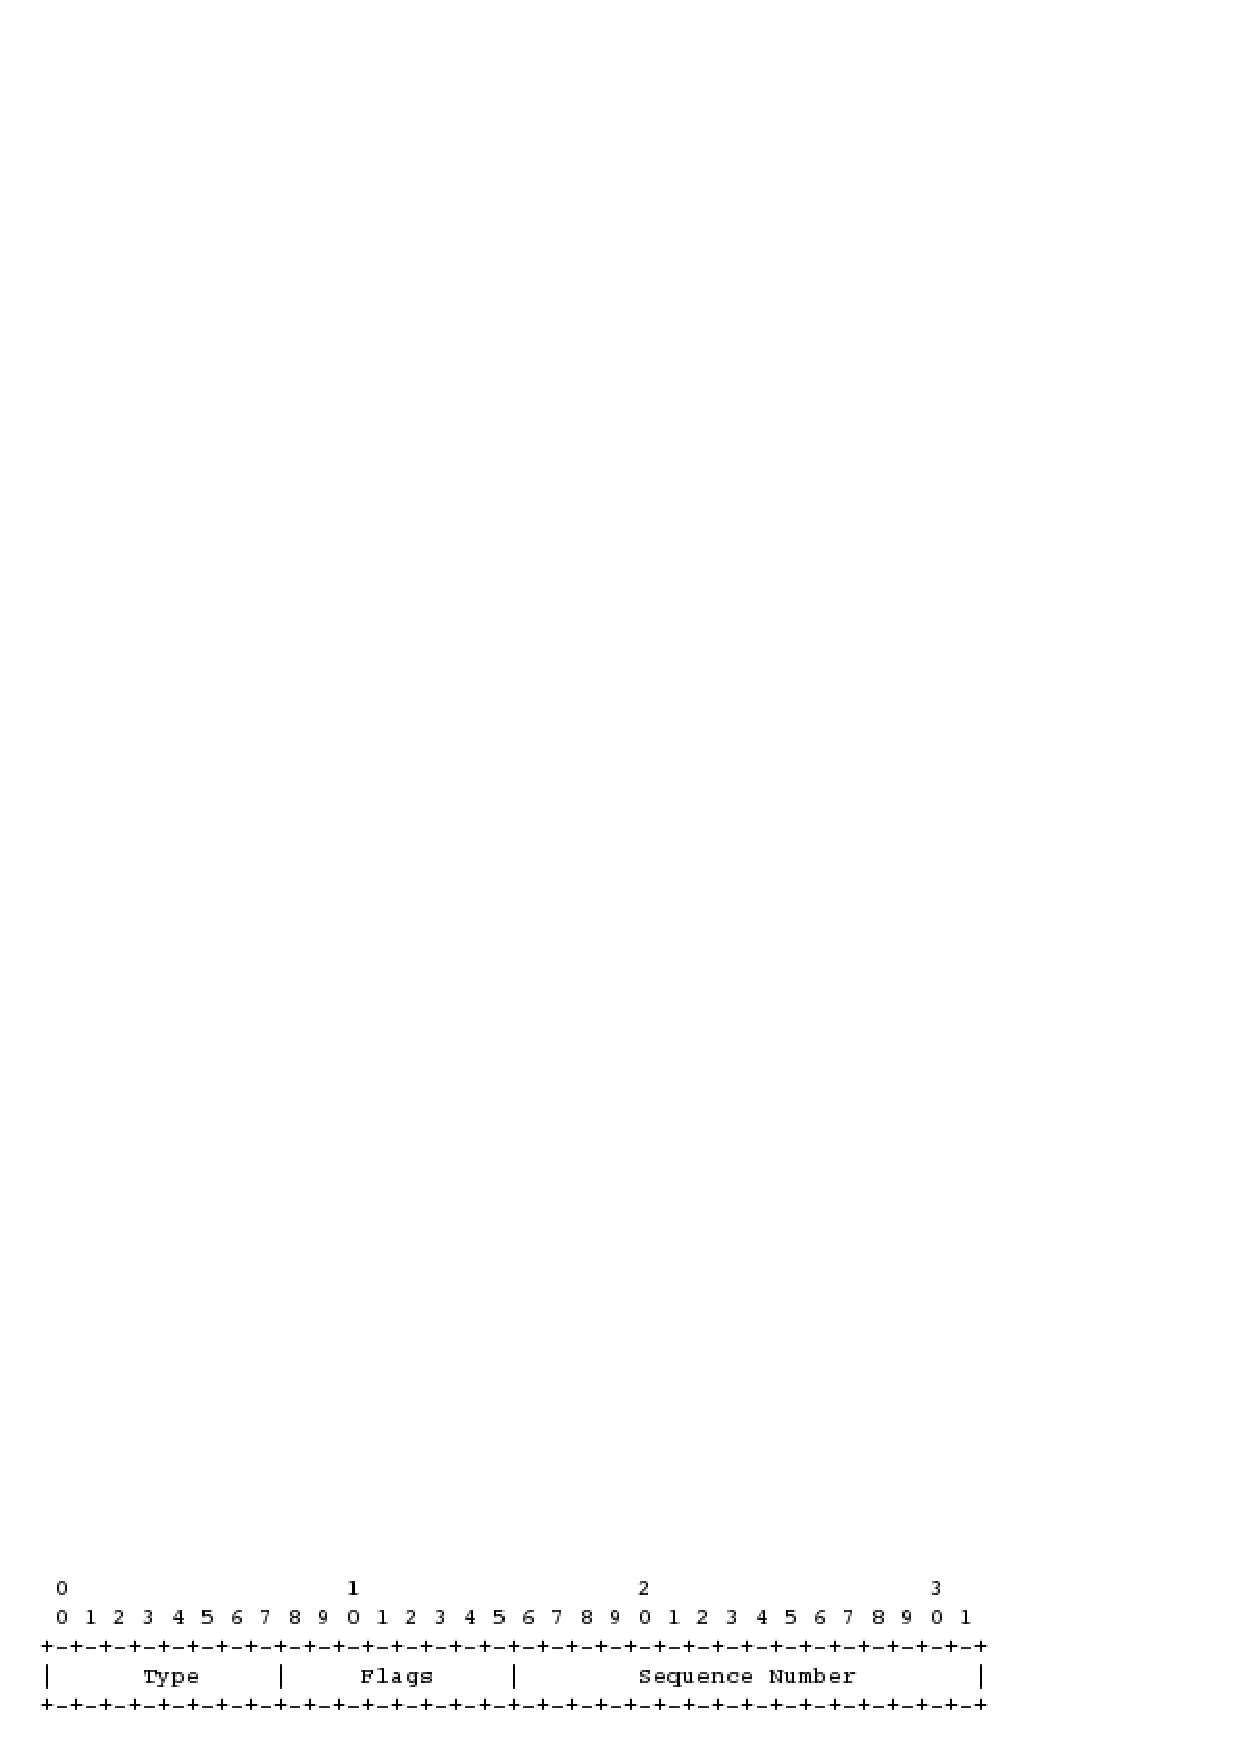
\includegraphics[scale=0.7]{img/snm-hdr.pdf}
\caption{SNM Message Header \label{img:snm-hdr}}
\end{center}
\end{figure}

\subsection{SNM Request Message}
\label{sub-sec:snm-request}
The request message flags have the following meanings:
\begin{itemize}
\item \emph{S} – all known SNM addresses of running supernodes are requested.
\item \emph{C} – all communities coordinated by the receiving supernode are requested.
\item \emph{N} – only SNM addresses of supernodes coordinating the provided communities are requested. The request payload will contain a list of community names. Every community name is filled as a variable-length name (name length followed by the string itself). \emph{N} and \emph{C} flags are mutually exclusive.
\item \emph{A} – the advertise address (N2N supernode address) is requested.
\item \emph{E} – message is initiated by an edge-node.
\end{itemize}

\begin{figure}[hbtp]
\begin{center}
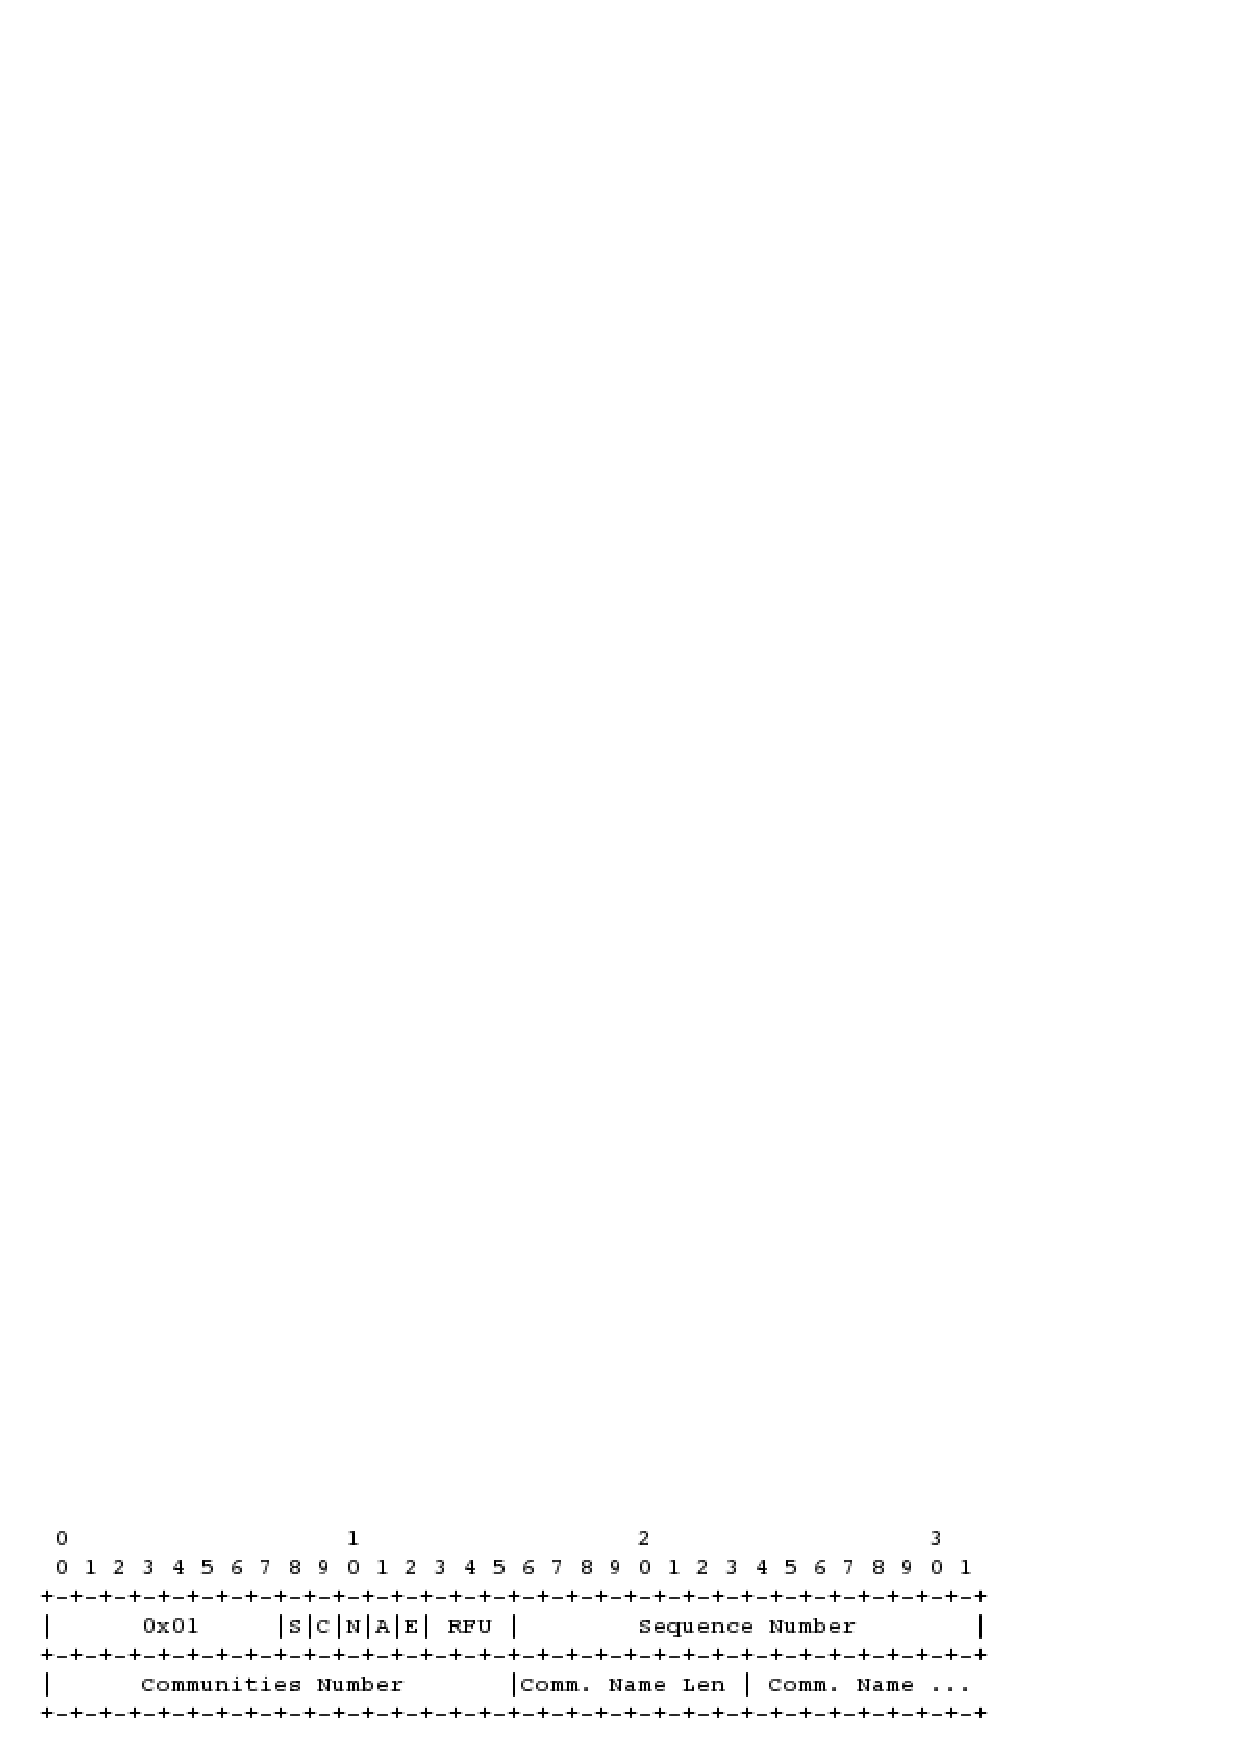
\includegraphics[scale=0.7]{img/snm-req.pdf}
\caption{SNM Request Message \label{img:snm-req}}
\end{center}
\end{figure}

\subsection{SNM Response Message}
\label{sub-sec:snm-response}
\labelindexref{Fig.}{img:snm-rsp} represents the message format of the SNM response message. A SNM response is always sent by a supernode in reply to a SNM request. \emph{Supernodes Number} and \emph{Communities Number} fields will be always set, regardless the type of request that was previously sent.
The supernodes addresses are encoded with the following fields:
\begin{itemize}
\item \emph{Family} – 1-byte value representing the IP protocol family (IPv4 or IPv6)
\item \emph{UDP Port} – 2-bytes value 
\item \emph{IP Address} – 4-bytes IPv4 address or 16-bytes IPv6 address 
\end{itemize}

\begin{figure}[hbtp]
\begin{center}
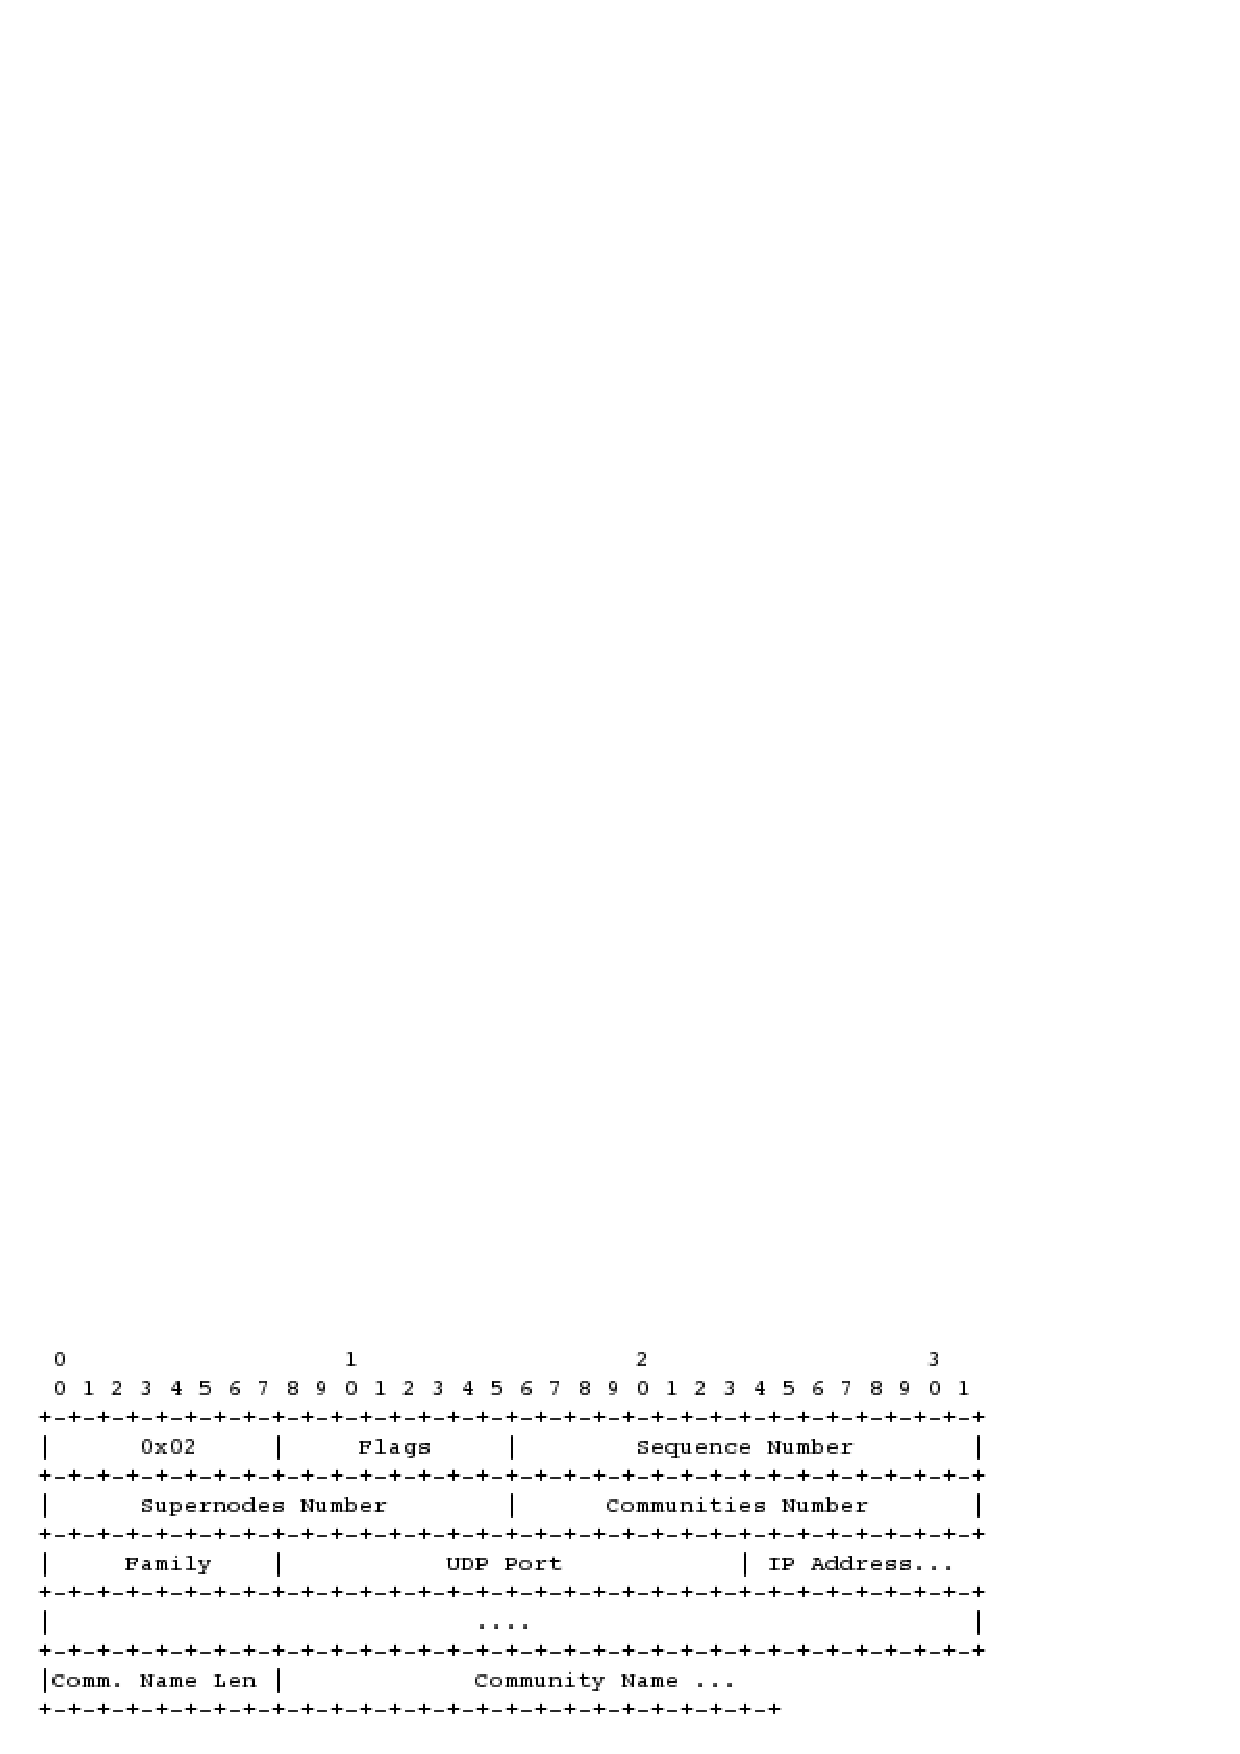
\includegraphics[scale=0.7]{img/snm-rsp.pdf}
\caption{SNM Response Message \label{img:snm-rsp}}
\end{center}
\end{figure}

If \emph{S} flag is set the response will contain SNM addresses of all known supernodes. If \emph{A} flag is set then the response will contain advertise addresses (N2N addresses) of supernodes coordinating a provided community. If \emph{N} flag is set, the supernodes addresses in the response are associated with an included community name. If \emph{C} flag is set, then the community names included in response are all those coordinated by responding supernode. If the response is sent to an edge-node, then when \emph{C} flag is set, only the community number is provided, considering that an edge will have no interest in other coordinated communities.

\subsection{SNM Advertise Message}
\label{sub-sec:snm-advertise}
The advertise message contains the advertise address of sending supernode and the names of communities coordinated by it. If the message is sent to another supernode, it may have the \emph{A} flag set, stating that sending supernode is also requesting for its counter-party advertise address. This may only happen during the community discovery stage of a starting supernode. A receiving supernode will advertise the sender in the registration acknowledgments sent to edges.

\begin{figure}[hbtp]
\begin{center}
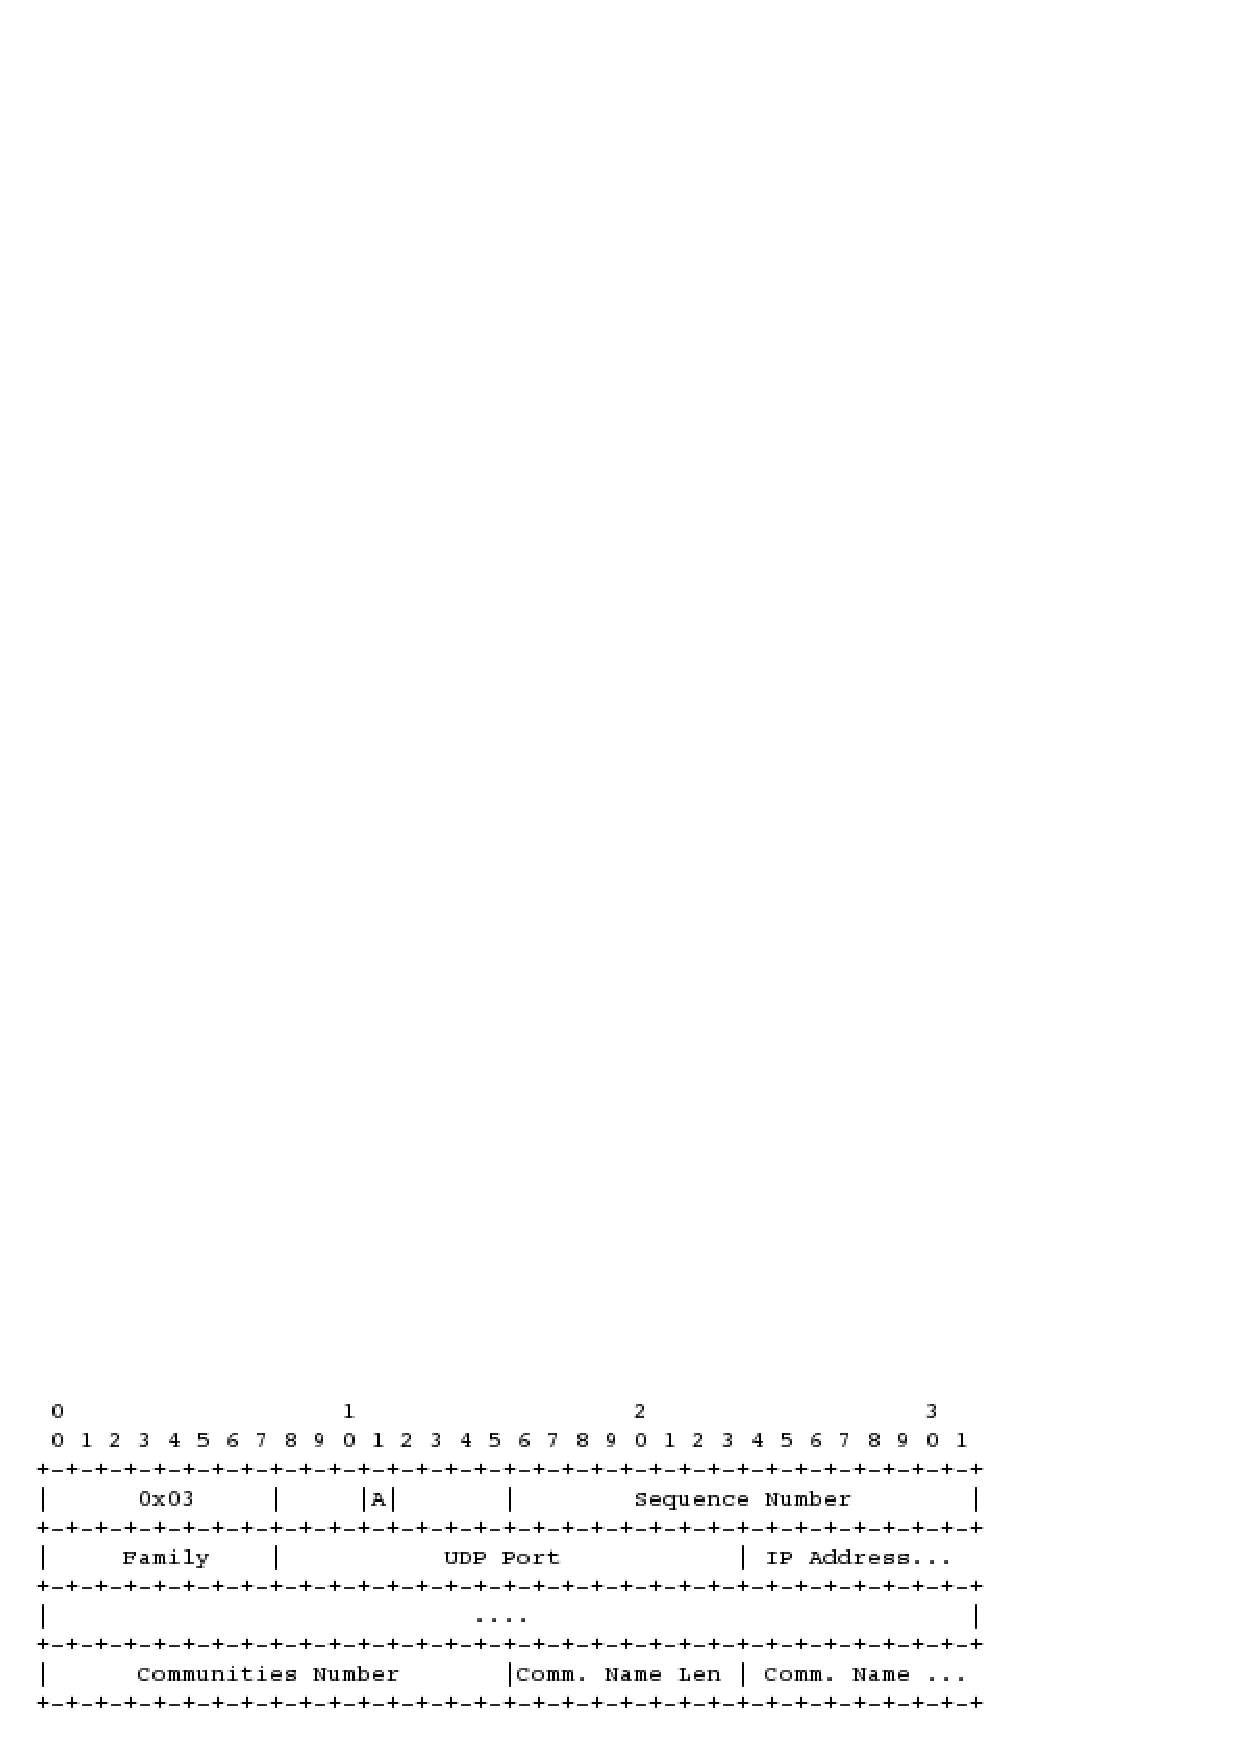
\includegraphics[scale=0.7]{img/snm-adv.pdf}
\caption{SNM Advertise Message \label{img:snm-adv}}
\end{center}
\end{figure}